\documentclass[final]{beamer}
\mode<presentation> {
	\usetheme{wtsi}
}
\usepackage[english]{babel}
\usepackage[latin1]{inputenc}
\usepackage{amsmath,amsthm, amssymb, latexsym}
\usepackage{tikz}
\usetikzlibrary{shapes.geometric, arrows}
\usepackage[orientation=portrait,size=a0,scale=1.4,debug]{beamerposter}
\usefonttheme[onlymath]{serif}
\boldmath
 
\title{Using haploid human DNA to design and evaluate the HiSeq X data processing strategy}
\author{Martin O. Pollard, Thomas M. Keene, Shane A. McCarthy, Joshua C. Randall, Richard M. Durbin}
\institute[Wellcome Trust Sanger Institute]{Wellcome Trust Sanger Institute}
\date{Today}

\begin{document}
\begin{frame}{}
    \begin{columns}
    % ---------------------------------------------------------%
    % Set up a column 
    \begin{column}{.49\textwidth}
        \begin{beamercolorbox}[center,wd=\textwidth]{postercolumn}
            \begin{minipage}[T]{.95\textwidth}  % tweaks the width, makes a new \textwidth
            \begin{block}{Introduction}
            The Illumina HiSeq X promises a reduction in sequencing cost but has required changes to the chemistry, software, and output.  To take advantage of this we have designed experiments using well characterised samples to explore what we need to do to best take advantage of these improvements. 
            \end{block}
            \begin{block}{Workflow}
                \tikzstyle{io} = [trapezium, trapezium left angle=70, trapezium right angle=110, minimum width=3cm, minimum height=1cm, text centered, draw=black, fill=blue!30]
                \tikzstyle{process} = [rectangle, minimum width=9cm, minimum height=3cm, text centered, draw=black, fill=orange!30]
                \tikzstyle{decision} = [diamond, minimum width=9cm, minimum height=3cm, text centered, draw=black, fill=green!30]
                \tikzstyle{arrow} = [thick,->,>=stealth]
                \centering
                \begin{tikzpicture}[node distance=4.5cm]
                    \node (in1) [io] {Illumina RTA};
                    \node (pro1) [process, below of=in1] {Mapper};
                    \node (pro2) [process, below of=pro1] {Fix Mate Pairing};
                    \node (pro3) [process, below of=pro2] {Sort};
                    \node (pro4) [process, below of=pro3] {Mark Duplicates};
                    \node (pro5) [process, below of=pro4] {Call};
                    \node (pro6) [process, below of=pro5] {Normalise variants};
                    \node (dec1) [decision, below of=pro6, yshift=-1.5cm] {Evaluate};
                    \draw [arrow] (in1) -- (pro1);
                    \draw [arrow] (pro1) -- (pro2);
                    \draw [arrow] (pro2) -- (pro3);
                    \draw [arrow] (pro3) -- (pro4);
                    \draw [arrow] (pro4) -- (pro5);
                    \draw [arrow] (pro5) -- (pro6);
                    \draw [arrow] (pro6) -- (dec1);
                \end{tikzpicture}
            \end{block}
            \begin{block}{Method}
              In order to test the importance of the reference on our data we tested: 
                \begin{itemize} \itemindent80pt
                    \item 1000 Genomes Phase II reference - hs37d5
                    \item GRCh38 analysis reference without alts.
                \end{itemize}
              And the following callers:
                \begin{itemize} \itemindent80pt
                    \item Samtools and BCFtools 1.1
                    \item GATK Haplotype Caller 3.2
                \end{itemize}
              These were evaluated against:
                \begin{itemize} \itemindent80pt
                    \item NIST Genome in a Bottle 0.2
                \end{itemize}
                Unfortunately no Genome in a Bottle release was available for build 38 of the Human Reference, so we had to lift this resource over using the UCSC chain files.
            \end{block}
            \begin{block}{Results}
\begin{tabular}{|l|c|c|c|}
\hline
Pipeline & Called (TP) & In in GIAB(FP) & Not Called (FN) \\ \cline{1-4}
38M 13350 Samtools 1.1 & 62919 & 2937 & 701 \\ \cline{1-4}
38M 13502 Samtools 1.1 & 62895 & 2890 & 725 \\ \cline{1-4}
38M 13350 GATK HC 3.2 & 62883 & 2911 & 737 \\ \cline{1-4}
38M 13502 GATK HC 3.2 & 62824 & 2768 & 796 \\ \cline{1-4}
38M Illm Plat GATK HC 3.2 & 62878 & 2792 & 742 \\ \cline{1-4}
37M 13350 Samtools 1.1 & 63249 & 2721 & 703 \\ \cline{1-4}
37M 13502 Samtools 1.1 & 63224 & 2686 & 728 \\ \cline{1-4}
37M 13350 GATK HC 3.2 & 63211 & 2693 & 741 \\ \cline{1-4}
37M 13502 GATK HC 3.2 & 63153 & 2585 & 799 \\ \cline{1-4}
\hline
\end{tabular}
            \end{block}
            \vfill
          % ---------------------------------------------------------%
          % end the column

            \end{minipage}
        \end{beamercolorbox}
    \end{column}
        \begin{column}{.49\textwidth}
        \begin{beamercolorbox}[center,wd=\textwidth]{postercolumn}
            \begin{minipage}[T]{.95\textwidth}  % tweaks the width, makes a new \textwidth
            \begin{block}{}
                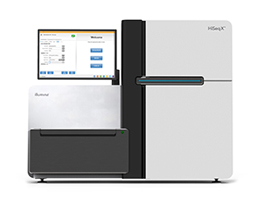
\includegraphics[width=.95\linewidth]{images/hiseq-x}
            \end{block}
            \begin{block}{What has changed?}
                \begin{itemize} \itemindent50pt
                    \item Error Profile (particularly context specific errors).
                    \item Quality Score Binning by default.
                    \item Read length increased to 150bp.
                    \item New Mappers available and required to take advantage of read length.
                \end{itemize}
            \end{block}
            \begin{block}{Conclusions}
                It appears that lifting over the variants between GRCh37 and GRCh38 introduced a small bias into our results, however our results do appear to confirm that the switch between these builds does not appear to affect the variants called to a large degree.
            \end{block}
            \begin{block}{Future work}
                Owing to deadlines and limits on computational resources the BWA backtrack and SNAP aligners were not included in this verison of the evaluation. For the final write up these results will be included and compared.  Also since this work was started a new version of BWA has been proposed that supports mapping to alternate haplotypes, given that much of the genomic material from the 1000 Genomes phase II reference decoys were incorporated into these we expect it to make a material difference to our mappings. We therefore propose to extend our analysis to incorporate an evaluation of the effects of mapping to these additional sequences.
            \end{block}
            \begin{block}{Acknowledgements}
                Sanger Core Sequencing Team for providing the data. Sanger NPG for quality control. Tommy Carsten for 
            \end{block}
            \vfill

          % ---------------------------------------------------------%
          % end the column

            \end{minipage}
        \end{beamercolorbox}
    \end{column}
    \end{columns}

\end{frame}
\end{document}

